
\section{既存の言語パターンマッチシステムの概要と改善点}



%本章では既存のパターンマッチシステムの全体像と,改善が必要な問題点について述べ
%る.2.1節で既存のパターンマッチシステムの全体像について述べ,2.2節に既存のシステムの問題点を挙げ,2.3節では2.2節で挙げた問題点に対する改善案について説明をする.

This chapter describes the overall picture of the existing pattern matching system and the problems that need to be improved. Section 2.1 describes the overall picture of the existing pattern matching system, Section 2.2 lists problems with the existing system, and Section 2.3 describes proposed improvements to the problems listed in Section 2.2.


\subsection{既存の言語パターンマッチシステムの全体像}

%本節では既存のパターンマッチシステムの全体像について説明する.既存のパターンマッチシステムを図\ref{figure:1}
%に示す.
%既存のパターンマッチシステムは情報を抽出したいテキスト文を解析し,その解析結果から,ユーザ自らが対象に予め関係する文や文の一部に対応する文構造のパターンを用意し,パターンに合致する結果を取得するというものである.実際の処理の流れは図\ref{figure:2}に記載してある.

This section describes the overall picture of the existing pattern matching system. The existing pattern-matching system is shown in Figure 1.
Figure 1 shows the existing pattern matching system.
Existing pattern matching systems analyze text sentences from which information is to be extracted, and from the analysis results, users prepare patterns of sentence structures corresponding to sentences or parts of sentences related to the target in advance, and obtain results that match the patterns. The actual flow of the process is shown in Figure%\ref{figure:2}.
\begin{figure}[htbp]
\centering
%\includegraphics[width=100mm]{figure1.png}
\caption{既存のパターンマッチシステムの構成図}
\label{figure:1}
\end{figure}
\begin{figure}[htbp]
\centering
%\includegraphics[width=100mm,scale=0.5]{figure2.png}
\caption{既存のパターンマッチシステムの処理の流れ}
\label{figure:2}
\end{figure}
%既存のシステムはユーザが実際に操作するフロントエンドと,フロントエンドから受け取ったデータを処理するバックエンドで構成される.その詳細を以下の\ref{sec:2-1-1}節,\ref{sec:2-1-2}節で説明する.
Existing system is a front that the user actually operates. The system consists of a front end and a back end that processes data received from the front end.
The details are described in sections 2.1.1 and 2.1.2 below.

\subsubsection{フロントエンド}
\label{sec:2-1-1}
%フロントエンドは主にJavaScriptのフレームワークReactを用いて構築しており,以下のような機能を有している.
The frontend is mainly built using the JavaScript framework React, and has the following functions.

\begin{description}
   \item[コーパスアップロード]\mbox{}\\
%解析対象のコーパスファイルのアップロードを行う.文の区切りは句点,感嘆符お
%よび疑問符で認識される.
Upload the corpus file to be analyzed. Sentence breaks are recognized by punctuation marks, exclamation points
and question marks.
   \item[コーパス解析結果表示]\mbox{}\\
%以下の図\ref{corpus_results}のようなコーパスの解析結果を表示する.

\begin{figure}[htbp]
 \begin{minipage}[b]{0.45\linewidth}
    \centering
    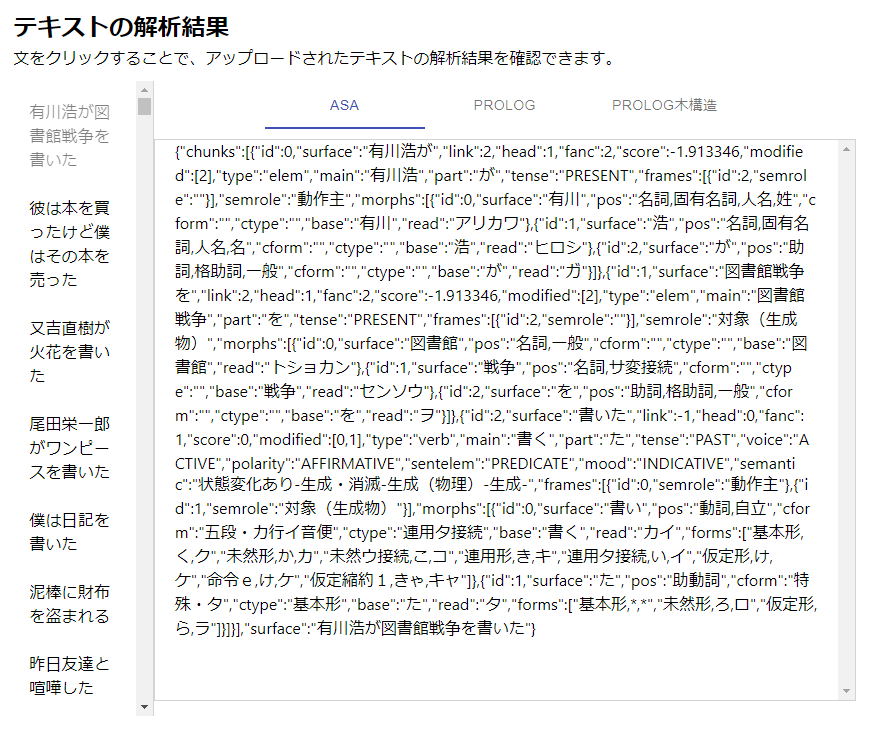
\includegraphics[scale=.4]{figure/asa_results.png}
  \subcaption{ASA}\label{figure:3-1}
  \end{minipage}
  \begin{minipage}[b]{0.45\linewidth}
    \centering
    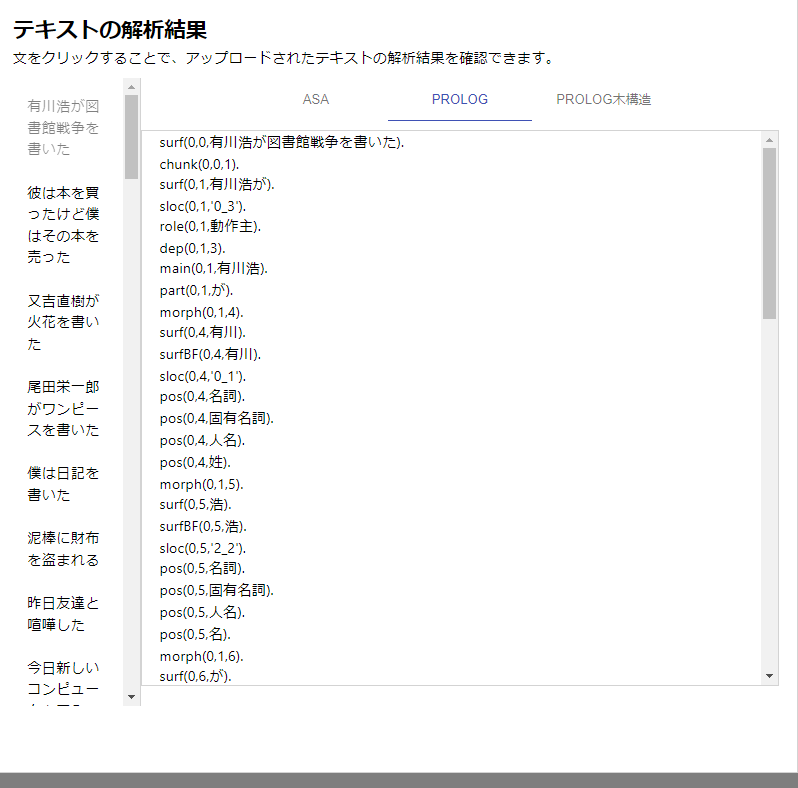
\includegraphics[keepaspectratio, scale=0.4]{figure/prolog.png}
    \subcaption{Prolog}\label{figure:3-1}
  \end{minipage}
  \begin{minipage}[b]{0.45\linewidth}
    \centering
    \includegraphics[keepaspectratio, scale=0.5]{figure/prolog木.png}
    \subcaption{木構造}\label{figure:3-2}
  \end{minipage}
  \caption{解析結果の表示}\label{corpus_results}
\end{figure}


\item[言語パターン構築]\mbox{}\\
%Blocklyを用いて視覚的にブロックを組み合わせることで検索したい言語パターンを構築することがで
%きる.多種のブロックを組み合わせることにより,ASAの解析結果の情報を複雑に
%検索することができる.図\ref{blockly:1}は著者と作品を抽出する言語パターンである.
Using Blockly, you can construct the language pattern you want to search for by visually combining blocks.
By combining many different types of blocks, the information in the ASA analysis results can be complex. By combining many different types of blocks, it is possible to search for information on ASA parsing results in complex ways.
Figure 1. Figure is a language pattern for extracting authors and works.

\begin{figure}[htbp]
  \centering
  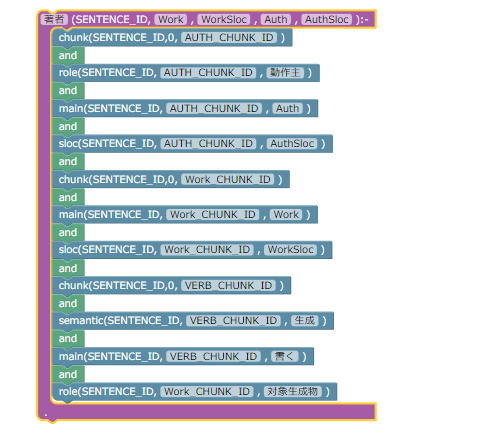
\includegraphics[scale=.3]{figure/make_pattern.png}
  \caption{Blocklyによる「著者」と「作品」を抽出する言語パターン}
  %\label{blockly}
\end{figure}

%また構築した言語パターンを xml 形式のファイルにエクスポートすることができる.エク
%スポートしたファイルをインポートすることもできる.
It is also possible to export the constructed language patterns to xml format files.
The exported file can also be imported.
\item[言語パターンマッチ結果表示]\mbox{}\\
%言語パターンマッチの実行結果を表示する.表示形式には,KWIC 形式,強調形式,
%テーブル形式がある.図\ref{blockly:1}の言語パターンを検索クエリとして言語パターンマッチを実行した結果が図\ref{display_result}である.AuthSlockは作品,WorkSlocは著者を意味しており,それぞれの形式でコンコーダンス表示されている.
Displays the results of language pattern matching. The display format includes KWIC format, highlighting format, and
table format. Figure  shows the result of executing language pattern matching using the language pattern in Figure 

\begin{figure}[htbp]
 \begin{minipage}[b]{0.45\linewidth}
    \centering
    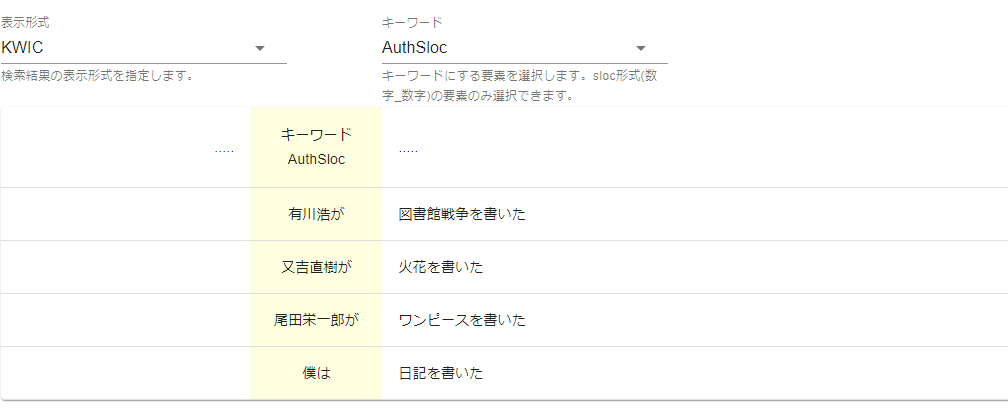
\includegraphics[keepaspectratio, scale=0.4]{figure/KWIC_results.png}
    \subcaption{KWIC}\label{figure:KWIC}
  \end{minipage}
  \begin{minipage}[b]{0.45\linewidth}
    \centering
    \includegraphics[keepaspectratio, scale=0.4]{figure/csent_results.png}
    \subcaption{強調}\label{figure:acsent}
  \end{minipage}
  \begin{minipage}[b]{0.45\linewidth}
    \centering
    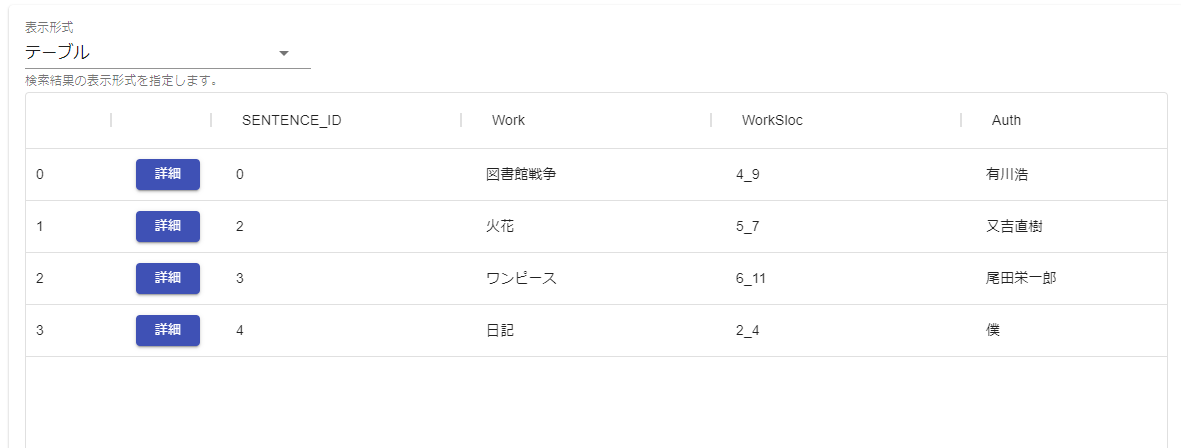
\includegraphics[keepaspectratio, scale=0.4]{figure/table_results.png}
    \subcaption{テーブル}\label{figure:table}
  \end{minipage}
  \caption{言語パターンマッチ結果表示}\label{display_result}
\end{figure}
\end{description}




\subsubsection{バックエンド}
%バックエンドはPython Web フレームワークである Djangoで構築されている. ASAによる解析にはasapy, Prolog処理系にはprologpyを用いて実装されている.
The backend is built on Django, a Python web framework. It is implemented using asapy for analysis by ASA and prologpy for Prolog processing.
\label{sec:2-1-2}
\begin{description}
\item[コーパス解析]\mbox{}\\
%解析対象のコーパスを読み込み,ASA による解析, Prolog への変換を行う.
%生成した解析結果をフロントエンドに返却し,ブラウザのメモリに保存する.
Reads the corpus to be parsed, parses it with ASA, and converts it to Prolog.
The generated analysis results are returned to the front end and stored in the browser's memory.
\item[言語パターンマッチ]\mbox{}\\
%対象の Prolog と検索クエリに対し,Prolog 処理系によるクエリ検索を行う.
%生成したパターンマッチ結果をフロントエンドに返却し,ブラウザのメモリに保存する.
Query the target Prolog and search query using the Prolog processor.
The generated pattern matching results are returned to the front end and stored in the browser memory.
\end{description}


%%%コメントアウト%%%%%
\begin{comment}
\subsection{既存のシステムの問題点}
\label{sec:2-2}
本節では,既存のパターンマッチシステムの問題点について大きく2つ説明する.

一つ目の問題としては英語を含んだ文のパターンマッチができないことである.現在のパターンマッチで利用しているProlog処理系はPythonで作成した簡易版であるため,ANDやORなどの英語の論理演算子のような特定の単語の入力を受け付けないからである.将来的に複雑なテキストを処理する際にボトルネックとなるため,このような問題を解決するための別の処理系の実装が求められる.

二つ目の問題としては大規模のコーパスの入力を受け付けないことである.現在のパターンマッチシステムでは1度に解析できる文数に限度があり,1000文のテキストを解析することでさえ約20分以上かかり,5000 文以上のテキストをアップロードして解析しようとすると動作が止まってしまう.
現在のシステムでは,解析結果返却の際に,テキストデータをブラウザのメモリに保存しているため.大規模なコーパスの入力を受け付けない.またその言語パターンマッチをバックエンド側で行う際にテキストデータを再送信しているためフロントエンドとバックエンドの通信する回数やデータ量が多くなってしまうため,動作時間が増加している.このような問題を解決するためにデータベースを導入するなどテキストデータの保存先の変更することにより,大規模なテキストコーパスでも解析およびパターンマッチで動作可能にし,動作時間をさらに向上することが求められる.
\subsection{言語パターンマッチシステムの改善点の整理}
\label{sec2-3}
本節では,既存のパターンマッチシステムの改善案について整理する.\ref{sec:2-2}節の問題を受け,以下のような改良案が挙げられる.以降の章で詳細を述べる.
\begin{itemize}
\item 既存のProlog処理系をSWI-Prologに変更する
\item データベースとしてElasticsearchを導入する

\end{itemize}
\end{comment}